\documentclass[sigplan,screen,sigconf]{acmart}
\usepackage{tcolorbox}
\usepackage{minted}
\settopmatter{printfolios=false,printacmref=false}
\bibliographystyle{ACM-Reference-Format}

\setcopyright{rightsretained}
\acmDOI{}
\acmISBN{}
\acmConference[LATTE '25]{Workshop on Languages, Tools, and Techniques for Accelerator Design}{March 30, 2025}{Rotterdam, Netherlands}

\author{Samit Basu}
\affiliation{
  basu.samit@gmail.com
  \country{Fremont CA, USA}
}

\begin{document}

\title{RHDL me this: Can Rust be a Hardware Description Language?}

\begin{abstract}
In \cite{b13} I began making the case that Rust is an excellent language for hardware description.  The initial attempt
descripted in that paper was published as RustHDL \cite{b6} and commercially deployed products have been developed using
RustHDL.  However, feedback from developers learning RustHDL revealed several weaknesses in the design.  As a result, 
I designed RHDL \cite{b10}, which is a complete rewrite of RustHDL that attemps to address these shortcomings and significantly 
expand the capabilities of the tool.
\end{abstract}

\maketitle

\section{Introduction}

In my prior paper, I described the various reasons that Rust makes an excellent choice for a hardware description language.  This included the strong typing, functional programming language features, package management and tooling, support for generics and a strong open source ecosystem. I also described the RustHDL framework, which transforms a carefully selected subset of Rust
into synthesizable Verilog.  Within a set of implicit rules, gateware could be built using Rust code.  There were, however, several shortcomings that became apparent as more engineers began to use RustHDL.  
The complete list of new features is too long to list here, but I will focus on the following key items:

\begin{itemize}
\item Algebraic Data Types (also called Sum types, or enums with data).
\item Type inference and local variable support.
\item Early returns, match and if expressions.
\item Timing estimation and analysis.
\end{itemize}

Achieving these features has required the introduction of a new co-compiler that runs in parallel to `rustc` to analyze the Rust source code and generate a series of HDL-compatible representations that are successively lowered towards hardware. Both compilers work together to ensure that the language invariants are met at all stages, and that undefined behavior is prevented.

\section{Syntax}
RHDL (like it's predecessor RustHDL) is embedded in the Rust programming language, much as 
MyHDL is embedded in Python\cite{b3} and Chisel is embedded in Scala \cite{b2}.  As a result,
all RHDL code must be valid Rust and must meet all the requirements of the Rust compiler.  This design means an entire class of errors are eliminated, as the language enforces correct usage of types, prevents use-before-initialization, unassigned outputs, etc.  Furthermore, by using Rust itself, as opposed to something Rust-like or a DSL \footnote{Both Spade \cite{b1} and XLS \cite{b4} use a Rust-inspired syntax for hardware description.} all the tools that work with Rust can be used with RHDL unmodified.  Of course, the challenge with this approach is that only a very small set of Rust code can be directly mapped to Verilog.  Each extension requires significant analysis of the underlying code to enable the relevant transformations.  A brief summary of some of the more significant changes follows.

\subsection{Algebraic Data Types}
The main request from RustHDL users was support for Algebraic Data Types. These are essentially tagged unions, where the tag is created and tracked by the compiler, \emph{and it is guaranteed to be a valid combination of tag and data}.  This is an incredibly powerful feature in Rust that RustHDL was unable to support due to lack of any direct equivalent in Verilog.  In RHDL, however, ADTs are supported, and are essentially unrestricted in their use.  For example, the following can be used in synthesizable designs:
\begin{minted}[fontsize=\footnotesize]{rust}
  enum MyEnum {
    // No payload
    A, 
    // A 4-bit payload and a 6-bit payload
    B(b4, b6),
    // A named payload, one field is a 3-element array
    // of 2-bit values.
    C{ x: b4, y: b6, z: [b3; 3] }, 
  }
\end{minted}
All of these \emph{variants} are stored in a union that will be sized large enough to store the largest variant and discriminant.  In this case, the type is 21 bits wide.  RHDL can create a layout diagram to illustrate the layout of the enum:
\begin{figure}[h]
  \centering
  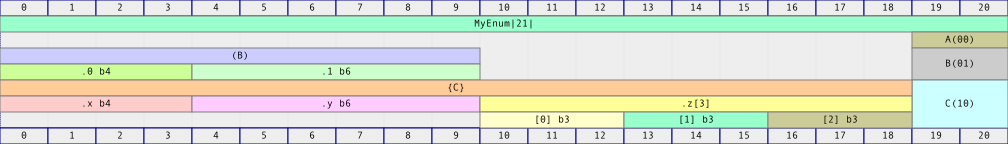
\includegraphics[width=8.5cm]{my_enum.png}
  \caption{Autogenerated layout of the MyEnum enum in RHDL}
\end{figure}
Using ADTs generally requires pattern matching and destructuring.  These are lowered into \verb|case| expressions automatically.  So for example:
\begin{center}
\begin{minipage}{3.8cm}
\begin{minted}[fontsize=\footnotesize]{rust}
  let w = MyEnum::B(1, 2);
  let v = match w {
    MyEnum::A => bits(1),
    MyEnum::B(a, ..) => a,
    MyEnum::C{ x, .. } => x,
  }
\end{minted}
\end{minipage}
$\rightarrow$
\begin{minipage}{4.1cm}
\begin{minted}[fontsize=\footnotesize]{rust}
  let w = MyEnum::B(1, 2);
  // Only valid if disc==1
  let a_if_w_is_B = __field(w, 0); 
  // Etc..
  let x_if_w_is_C = __field(w, "x");
  case __disc(w) {
    0 => y = bits::<4>(1),
    1 => y = a_if_w_is_B,
    2 => y = x_if_w_is_C,
  }
\end{minted}
\end{minipage}
\end{center}

\subsection{Type Inference and Local Variables}
The previous examples demonstrated the use of local variables and the commensurate need for type inference.  RHDL uses a simplified type inference pass to deduce and annotate the types of all variables in the original code.  This type pass \emph{must} agree with the types inferred by \verb|rustc| to avoid miscompilation.  Passes are included to ensure that all variables are typed by RHDL and that the typing is consisting with \verb|rustc|.  This trivial function is inferred as:
\begin{center}
\begin{minipage}{4cm}
\begin{minted}[fontsize=\footnotesize]{rust}
function(a: b4, b: b4) -> b4 {
  let x = 1;
  let y = (x, x + 1);
  y.0 + y.1
}
\end{minted}
\end{minipage}
$\rightarrow$
\begin{minipage}{4cm}
\begin{minted}[fontsize=\footnotesize]{rust}
  let a: b4;
  let b: b4;
  let x: b4;
  let y: (b4, b4);
  let _return: b4;
\end{minted}
\end{minipage}
\end{center}

In two cases, the \verb|RHDL| type inference is relied upon \emph{instead} of \verb|rustc|'s type inference.  The first is in the case of clock domains.  In \verb|RHDL|, a signal indicates the clock domain it belongs to by use of a type parameter (assigned a color).  So, for example, \verb|Signal<b4, Red>| indicates a nibble that changes on edges in the \verb|Red| clock domain, and \verb|Signal<b4, Blue>| signifies a nibble that changes in the \verb|Blue| clock domain.   Here is an example
which \verb|rustc| will pass, but \verb|RHDL| will flag as an error:
\begin{minted}[fontsize=\footnotesize]{rust}
  function(a: Signal<b4, Red>, b: Signal<b4, Blue>) 
     -> (Signal<b4, Red>, Signal<b4, Blue>) {
    let a = a.val(); // Extract the value of a
    let b = b.val(); // Extract the value of b
    let a = a + a;
    (signal(a), signal(b+a))
  }
\end{minted}
In this case, the \verb|.val| method strips the clock domain information from the signal (it has the signature \verb|Signal<T, C> -> T|), and
the \verb|signal| function has the signature \verb|T -> Signal<T, C>|.
But RHDL continues to track which values came from which clock domain, and emits the following error message:

\begin{figure}[h]
  \centering
  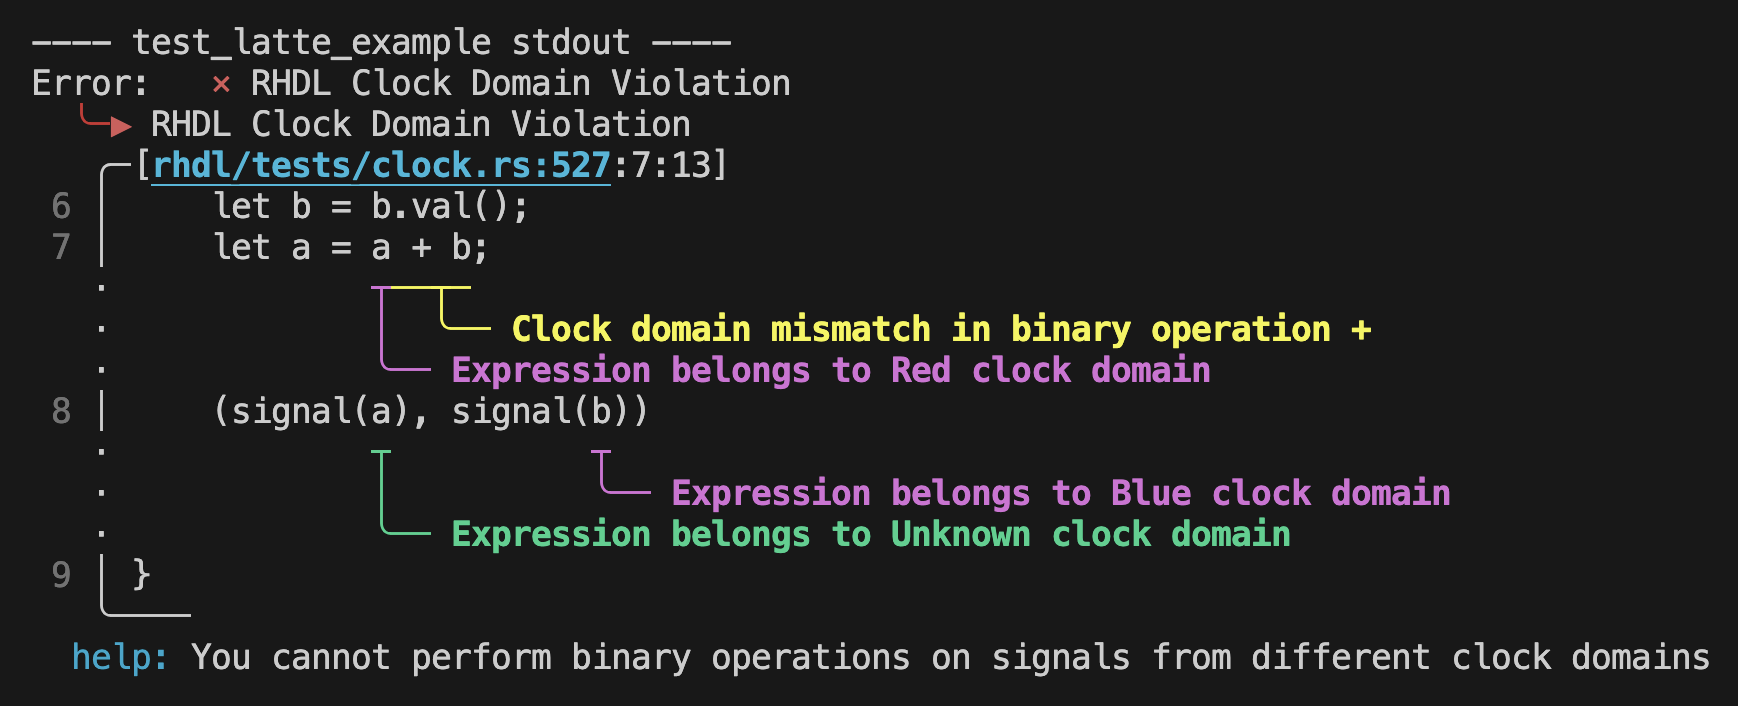
\includegraphics[width=8.5cm]{clock_error.png}
  \caption{Error message from RHDL indicating a clock domain error.}
\end{figure}

In this case, the clock domain information has been erased from the signals as far as \verb|rustc| is concerned (which is done to make the types reasonable to work with).  But the addition of signals from 
two separate clock domains is undefined in RHDL, hence the error.  The second instance in which type information is erased for \verb|rustc| but tracked for \verb|RHDL| is in the case of the DSP math operations.

\subsection{Expression Transformations}
Many Rust constructs are not directly mappable to Verilog.  For example, in Rust, all \verb|if| constructs are expressions, and can be used in any context where a value is expected.  Blocks also have values (in addition to side effects).  These are transformed into a series of mux expressions with renaming of local variables.

\begin{center}
  \begin{minipage}{0.25\linewidth}
    \begin{minted}[fontsize=\footnotesize]{rust}
      let mut z = 0;
      let x = if y {
        z += 1;
        z
      } else {
        z
      };
    \end{minted}
    \end{minipage}
    $\rightarrow$
    \begin{minipage}{0.60\linewidth}
  \begin{minted}[fontsize=\footnotesize]{rust}
    let z = 0;
    let z_if_y = z + 1;
    let z_if_not_y = z;
    let x = select(y, z_if_y, z_if_not_y);
    let z = select(y, z_if_y, z_if_not_y);
  \end{minted}
\end{minipage}
\end{center}
Note that the mutable variable is also removed by renaming.  In this case, type inference will also be required as the types of all of the variables are implicit.  Similar transformations are applied for things like \verb|match| expressions, and other flow control constructs.

\subsection{Timing Estimation}
A significant problem that arises in high level HDLs is the difficulty in fixing timing closure issues with the generated design.  This results from the very loose coupling between the design as expressed in the HDL and the resulting low level representation that feeds the synthesis tools.  RHDL includes a critical timing path estimator that can reference back to the source code, as in this example:

\begin{figure}[h]
  \centering
  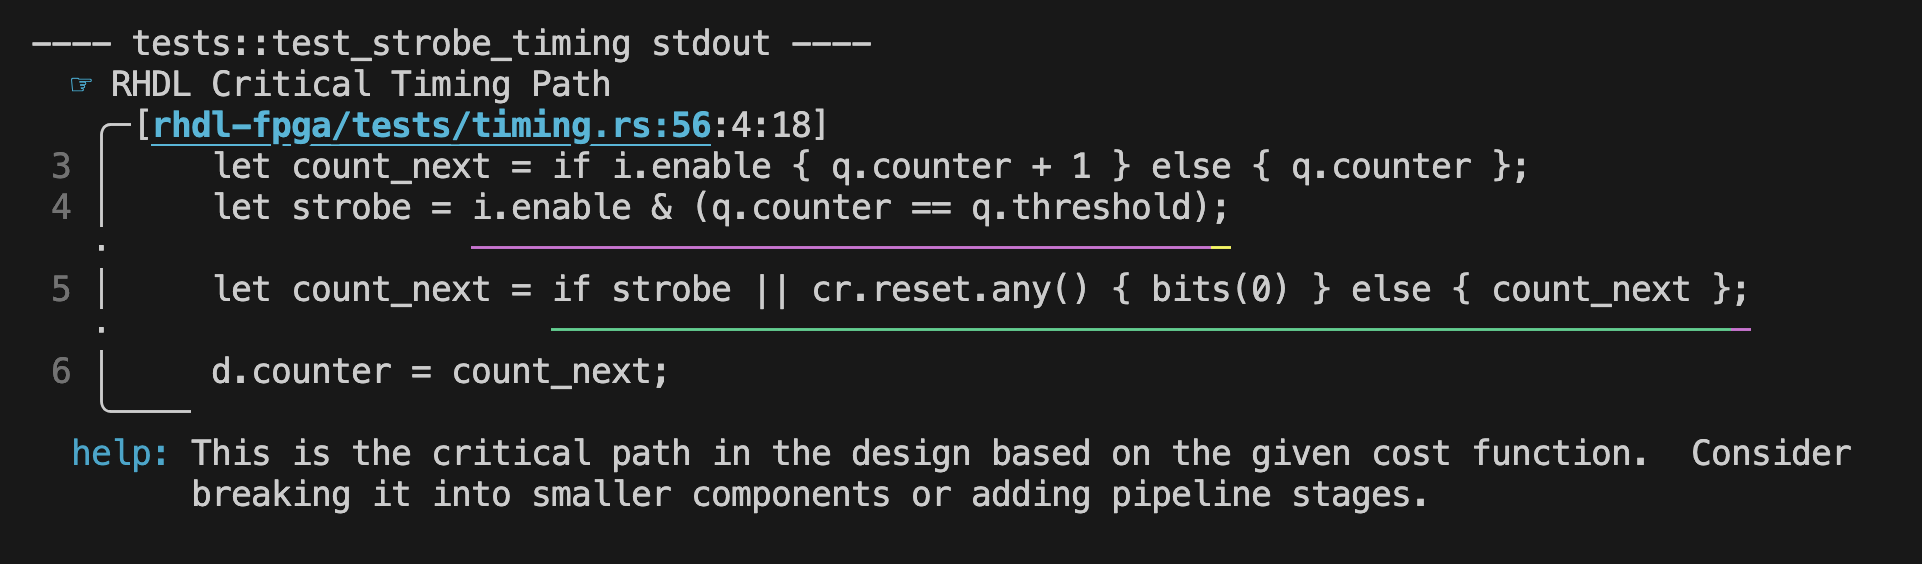
\includegraphics[width=8.5cm]{timing.png}
  \caption{Timing path estimation in RHDL}
\end{figure}

Although this is still crude compared to the analysis performed by the synthesis tools, it does provide a starting point for debugging timing issues.  A better solution would be for RHDL to annotate the generated design in such a way as to convert timing reports generated by 3rd party tools back into source code locations.  This is not currently possible.

\section{Simulation}

RHDL provides a graduated level of simulation capability that allows for increasing confidence in the correctness of a design as it is lowered from Rust to low level (synthesizable) Verilog.  These levels are:
\begin{itemize}
\item A pure Rust simulation that includes event-based simulation.
\item A Virtual Machine for the intermediate representation that preserves type information, but uses RTL constructs.
\item A Virtual Machine for the low level representation that discards type information and only manipulates bit vectors.
\item A flow graph model of the design that can be simulated in Verilog.  Used for timing estimation and various analysis passes (like logic loop detection).
\item A Verilog model that can be simulated with 3rd party tools.
\end{itemize}

Each of these levels can produce traces that can be viewed in \verb|surfer|.  A modified version of which can decode the structured type information included in the trace outputs to make debugging a better experience:

\begin{figure}[h]
  \centering
  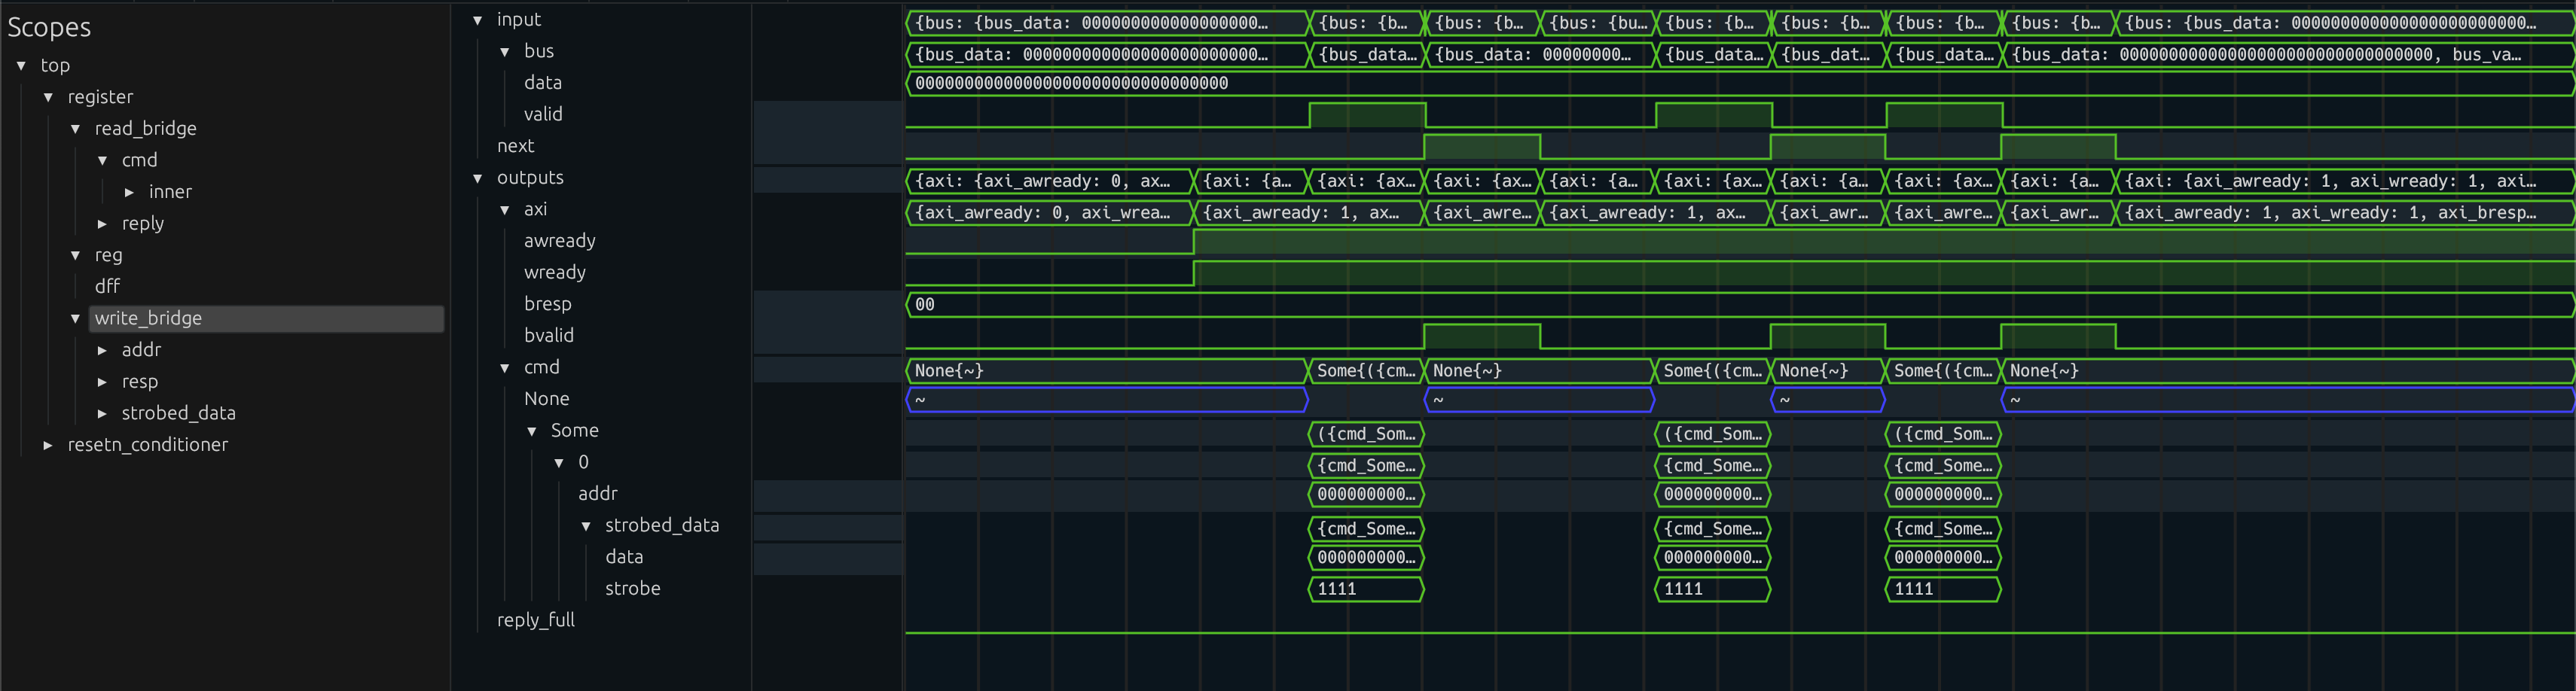
\includegraphics[width=8.5cm]{surfer.png}
  \caption{Surfer debugging a typed trace from the RHDL simulator}
\end{figure}


The RustHDL framework, and its successor RHDL, take advantage of all of these features to
create an environment for hardware description that is powerful, easy to use, extensible and open.  

The end goal is to enable a wider class of engineers to develop high quality hardware by reusing 
their skills as Rust developers in the hardware domain.  This paper briefly describes the RustHDL 
approach to developing FPGA firmware using the RPL, and then identifies the observed shortcomings
 and how they may be addressed in the upcoming RHDL framework.  Finally, I touch upon some of the
  unsolved problems in using Rust for hardware description.  Note that I use the term ``hardware description'' 
  here to mean FPGA firmware (or possibly ASIC designs), as Rust is already established as a language 
  for embedded systems programming (which is also often referred to as ``firmware''). 
I think it's also important to point out that the appeal of using Rust as an HDL is it's familiarity
 to engineers coming from a C background.  The syntax is ``C-like'', and
while functional programming concepts are supported, the language is multi-paradigm.  Given that part 
of the objective of RustHDL and RHDL is to enable a wider class of engineers to develop hardware, 
this is a critical point.

\section{Syntax}
RustHDL is not a new language.  Instead it is a set of libraries and macros along with a 
subset of the Rust programming language that can be used to generate firmware.  The key
principle of RustHDL is:

\begin{tcolorbox}
RustHDL designs are valid Rust programs that can be compiled and run on a host computer
using the included event-based simulator.
\end{tcolorbox}

In this sense, RustHDL is embedded in the Rust language much as MyHDL is embedded in Python \cite{b3},
and Chisel is embedded in Scala \cite{b2}.  
Note that unlike MyHDL, RustHDL does not use a generator pattern and infer the required hardware. 
 Instead, the AST itself is transformed into the circuit description.  For example, the following 
 AST fragment describes (behaviorally) a mux that selects between the current counter output 
 \verb|counter.q| and \verb|counter.q+1|.  The description is not ``builder'' style, in which a
  MUX is explicitly instantiated.  The MUX is inferred from the imperative code. 

\begin{minted}[fontsize=\footnotesize]{rust}
  // signal for false control signal --v
  self.counter.d.next = self.counter.q.val();
  //    v-- MUX control signal
  if self.enable.val() {
  // signal for true control signal  --v
    self.counter.d.next = self.counter.q.val() + 1;
  }
\end{minted}

This is in contrast to a combinator style of hardware description, for example in \cite{b4b}, where the 
language used is Rust, but hardware description is functional.

The syntax should be fairly familiar to anyone comfortable with Rust (or C++).  The 
following is an example of a simple SPI master in RustHDL, generic over the transaction size \verb|N|, edited for brevity:

\begin{minted}[fontsize=\footnotesize]{rust}
  #[derive(LogicBlock)]
  pub struct SPIMaster<const N: usize> {
      pub clock: Signal<In, Clock>,
      pub data_outbound: Signal<In, Bits<N>>,
      pub start_send: Signal<In, Bit>,
      pub data_inbound: Signal<Out, Bits<N>>,
      pub wires: SPIWiresMaster,
      local_signal: Signal<Local, Bit>,
      state: DFF<SPIState>,
      cs_off: Constant<Bit>,
  }
\end{minted}  

The \verb|pub| keyword is used to denote the visibility of the signals.  Signals 
marked with a direction, and type.  Internal components such as flip-flops and strobes
are all included in the top level struct, which is initialized using normal Rust code.
The \verb|Local| signal represents a local variable used in the update function, but
not otherwise exposed.  As RustHDL has no type inference, it requires explicit allocation
and types for all local variables.  The member \verb|cs_off| (along with others omitted) 
is a constant constructed at runtime that encodes the SPI mode of the bus.  Finally, 
the \verb|SPIWiresMaster| is a struct that describes the interface to the actual SPI bus.
Interfaces (unlike structs in SystemVerilog, for example) include both input and output
signals, and can be used to ``connect'' complex components with a single line.  

Note that in this instance, \verb|state: DFF<SPIState>| is equivalent to a module 
instantiation.  The \verb|DFF| is a flip-flop, and \verb|SPIState| is a C-style enum 
that represents the state of of the controller.  By including it as a member of the 
struct, we request an instance of it be created in the generated design.  Thus, composition of 
modules is equivalent to composition of data structures.

RustHDL (but \emph{not} RHDL) supports bidirectional interface declarations which can 
be used to connect complex components together in a type-safe way.
As an example, an interface to an SDRAM chip with a \verb|D-bit| data bus and a 13 bit 
address bus is defined as:

\begin{minted}[fontsize=\footnotesize]{rust}
  #[derive(LogicInterface, Clone, Debug, Default)]
  #[join = "SDRAMDriver"]
  pub struct SDRAMDevice<const D: usize> {
      pub clk: Signal<In, Clock>,
      pub we_not: Signal<In, Bit>,
      pub cas_not: Signal<In, Bit>,
      pub ras_not: Signal<In, Bit>,
      pub address: Signal<In, Bits<13>>,
      pub write_data: Signal<In, Bits<D>>,
      pub read_data: Signal<Out, Bits<D>>,
      pub write_enable: Signal<In, Bit>,
  }
\end{minted}

and can be connected to the corresponding signals in another IP block with a 
single \verb|join| statement.  This significantly reduces the amount of 
error-prone wiring that must be done by code or graphically.  The \verb|join| statement 
is used inside of an \verb|update| function as the following demonstration:

\begin{minted}[fontsize=\footnotesize]{rust}
#[derive(LogicBlock)]
struct I2CControllerTest {
    clock: Signal<In, Clock>,
    controller: I2CController,
    target_1: I2CTestTarget,
    target_2: I2CTestTarget,
    test_bus: I2CTestBus<3>,
}

impl Logic for I2CControllerTest {
    #[hdl_gen]
    fn update(&mut self) {
        clock!(self, clock, controller, target_1, target_2);
        I2CBusDriver::join(&mut self.controller.i2c, 
          &mut self.test_bus.endpoints[0]);
        I2CBusDriver::join(&mut self.target_1.i2c,
          &mut self.test_bus.endpoints[1]);
        I2CBusDriver::join(&mut self.target_2.i2c, 
          &mut self.test_bus.endpoints[2]);
    }
}
\end{minted}

In this example, the controller, and 2 DUTs are connected to a bus.  
Since all of the logic is simply connecting the interfaces together, 
it consists mainly of \verb|join| statements. 

Back to the SPI controller example, an update function calculates the next value of the 
signals (external and internal) based on the current state stored in the DFF \verb|state|,
which itself is a C-style enum.  Rust ensures that the state machine match/case is exhaustive. 

\section{Mental Model}
RustHDL attempts to build on HDLs like Lucid\cite{b11} to provide a more 
understandable mental model for how hardware works.  In an imperfect 
implementation, RustHDL defines a \verb|Signal| struct that has a read only 
endpoint \verb|x.val()| for signal \verb|x|, and a write endpoint \verb|x.next|.    
The comments indicate how the AST is transformed into a hardware description. 

\begin{minted}[fontsize=\footnotesize]{rust}
// Design is parametric over N - the size of the counter
impl<const N: usize> Logic for Strobe<N> {
  #[hdl_gen]
  fn update(&mut self) {
    // v-- latch prevention
    self.counter.d.next = self.counter.q.val();
    // v-- mux control signal
    if self.enable.val() {
      //  v-- value assigned to signal if mux control is true
      self.counter.d.next = self.counter.q.val() + 1;
    }
    // v-- combinatorial logic
    self.strobe.next = self.enable.val() & 
      (self.counter.q.val() == self.threshold.val());
    // v-- higher priority mux for previous mux output
    if self.strobe.val() {
      self.counter.d.next = 1.into();
    }
  }
} 
\end{minted}

Rust lacks write-only semantics, so the framework checks for read-before-write on the 
\verb|x.next| endpoint.  Using this nomenclature, the idea of non-blocking assignments 
is replaced with a conditional model - i.e., given the current value in the set of 
signals, what next value do I want them to take?  This mental model is coupled with 
analysis passes that look (with the aid of Yosys\cite{b12} in RustHDL) for latch 
inferences due to missing assignments and other such issues.

The mental model of RustHDL is not ideal (and is replaced in RHDL).  However, the main 
advantage it has is that it is very ``normal'' looking.  A signal's \verb|.next| endpoint 
can be written to as many times as desired inside of an \verb|update| function.  Only 
the last value it takes will matter when the function completes.  In essence, the last 
successful write to a signal ``wins'', where success may be conditional (in this case, 
for example, the value of \verb|self.counter.d.next| depends on the value of 
\verb|self.enable.val()|).  For synchronous logic this concept can be expressed as:

\begin{tcolorbox}
The current value of the signal is accessible via \verb|.val()|, and the value that 
signal will take on the next clock cycle will be decided by the last assignment
to \verb|.next|.  I.e., in the next clock cycle \verb| next -> val|.
\end{tcolorbox}

Note that in the case of asynchronous combinatorial logic, the value of a signal 
is defined when \verb|next| and \verb|val| are equal. Local variables can be both 
written to and read, functioning as scratchpads, as long as a write precedes any 
subsequent reads or writes.

RHDL simplifies the mental model by using the natural Rust data flow that arises
from functions operating on value types.  Data inputs are fed into functions, and
data outputs are returned, with the \verb|update| function becoming pure, with
no side effects. Feedback loops must be broken by registers.  I hope
to detail this more at the conference or in a future paper.


\section{Simulation}
Testing of designs in RustHDL does not require the use of third party tools or tooling.  
Tests utilize a built-in event-based simulation engine that can simulate any RustHDL 
design. Black box IP cores can be simulated by providing Rust equivalents of the 
hardware descriptions. The simplest example is something like a block RAM, which can 
be trivially instantiated in Verilog, but requires a behavioral model in RustHDL.  In 
RustHDL that behavioral model is written in Rust, and can be substituted into the 
simulation environment.  Other black box IP cores can be equivalently simulated in Rust. 
Note that because RustHDL supports combinatorial connections across modules that the
simulator iterates until it reaches a fixed point.  The iterations will terminate 
with an error if some upper limit is reached.

Speed is a critical factor in simulation.  RustHDL is a reasonably fast simulator, 
and the Rust test framework is inherently parallel, and can run multiple tests in 
parallel. Using system calls/shell-outs, the entire synthesis and bitstream generation
 process can be handled inside the Rust ecosystem.  A direct comparison with Verilator 
 proved difficult as Verilator rejected the Verilog generated by RustHDL (possibly due 
 to the presence of inter-module asynchronous logic in the design). 

\section{Reuse}
Hardware descriptions in RustHDL are simply \verb|struct|s, and are composed of other 
hardware components or modules via composition.  This allows for easy reuse of components, the
construction of complex designs out of simpler, smaller components, combined with 
sane rules of scoping and encapsulation.  Furthermore, each of the sub-components can be 
tested in isolation, and then tested after composition in the larger design. 

Rust is a very composable language, and \verb|crates.io| provides a natural mechanism
for sharing and reusing components.  As an example, in RustHDL, handling of hardware 
specific details (such as synthesis tools and constraints files for specific FPGAs and boards) 
is handled through a \emph{board support package}.  This is simple a library that provides the 
defaults, pin-outs, and other mapping information needed to generate a bitstream for a given 
piece of hardware.  As an open-ended and potentially unbounded problem, the BSP can be published 
as a \verb|crate| (package) in the Rust ecosystem by contributors \cite{b7}.  This decentralizes 
control over one of the more challenging parts of maintaining support for a bewildering array of devices. 

Meta-programming is supported in RustHDL, but to a somewhat limited extent.  Most of the 
meta-programming is provided by macros (procedural and declarative) that generate the 
necessary code.   FIFOs that require various generic parameters can be instantiated 
via a simple macro.  And interfaces use macros to describe mating interfaces with signals
of opposite direction.  

\section{Shortcomings and the Future}
RustHDL has been used for non-trivial commercial firmware development and is deployed.  
It has also seen some level of interest and adoption from the open source community.  
Feedback from early users lead to the following list of shortcomings:

\begin{itemize}
  \item The subset of Rust supported by RustHDL (which is the subset of the language 
  that can be directly translated into Verilog) is too small to write ``natural'' Rust code. 
  \item RustHDL does not support Algebraic Data Types (data-carrying enums).
  \item Local variables and type inference are critical to writing clean and
  idiomatic Rust code.  
  \item Composition of functions/behavior is not possible. 
  \item Writing test-benches required an understanding of the simulator mechanics.
  \item Backends are needed for more than just Verilog.
\end{itemize}

Solving all of these problems essentially necessitated a rewrite of RustHDL.  The
new framework, called RHDL (Rust Hardware Description Language) is currently under development.  
The primary technical difference to RustHDL is the introduction of an auxiliary compiler into 
the processing. This compiler works in tandem with \verb|rustc| to convert an AST of the code 
into a RTL-like HDL, and then transform and optimize that representation into a form that can
be synthesized.  The  compiler is key to support of things like early returns, match and 
if expressions (as opposed to statements), and other Rust-isms that are not common in
HDLs, but are common in Rust.  The compiler also provides ADT support with control 
over the layout of the data, and easy composition of data types into structs of arbitrary complexity.  

\begin{tcolorbox}
On unsolved problem that remains is the difficulty in connecting downstream toolchain
outputs (such as an analysis of a long-timing path) back to the original Rust code.  I believe
this is a significant problem for all high level HDLs and requires some serious thought, as
adoption by hardware engineers will be limited until the diagnostics from the downstream tools 
can be used to inform changes in the high level code.
\end{tcolorbox}

\section{Conclusions}
I believe Rust is a promising basis for a hardware description language.  It offers many powerful 
tools that can be utilized to build composable, reusable and correct hardware designs.  The RustHDL 
framework was a first step in this direction, and the in-development RHDL framework promises to address
many of the shortcomings of the first attempt.

\newpage

\begin{thebibliography}{00}
  \bibitem{b13} S. Basu, ``Rust as a Hardware Description Language'', LATTE 2024, San Diego, CA.
  \bibitem{b9} ``Rust - A language empowering everyone to build reliable and efficient software'', \url{https://rust-lang.org} (Accessed Feb 1, 2024).
  \bibitem{b1} F. Skarman and O. Gustafsson, ``Spade: An Expression-Based HDL With Pipelines'', Open Source Design Automation Conference, 2023.
  \bibitem{b4} ``XLS: Accelerated HW Synthesis'', \url{https://google.github.io/xls/} (Accessed Feb 1, 2024).
  \bibitem{b4b} Sungsoo Han, Minseong Jang, and Jeehoon Kang, ``ShakeFlow: Functional Hardware Description with Latency-Insensitive Interface Combinators'', ASPLOS 2023.
  \bibitem{b6} ``RustHDL - Write FPGA Firmware using Rust!'', \url{https://rust-hdl.org/} (Accessed Feb 1, 2024).
  \bibitem{b10} ``RHDL - Rust Hardware Description Language'', \url{https://github.com/samitbasu/rhdl} (Accessed Feb 1, 2024).
  \bibitem{b0} ``Stack Overflow Developer Survey 2023'', \url{https://insights.stackoverflow.com/survey/2023} (Accessed Feb 1, 2024).
  \bibitem{b3} ``MyHDL - From Python to Silicon!'', \url{https://www.myhdl.org/} (Accessed Feb 1, 2024).
  \bibitem{b2} ``Chisel - Software-defined hardware'', \url{https://www.chisel-lang.org/} (Accessed Feb 1, 2024).
  \bibitem{b11} J. Rajewski, ``Lucid - FPGA Tutorials'', \url{https://alchitry.com/lucid/} (Accessed Feb 18, 2024).
  \bibitem{b12} C. Wolf, ``Yosys Open SYnthesis Suite'', \url{https://yosyshq.net/yosys/} (Accessed Feb 18, 2024).
  \bibitem{b7} ``rust-hdl-bsp-step-mxo2-lpc - rust-hdl board support package for STEP-MXO2-LPC'', \url{https://crates.io/crates/rust-hdl-bsp-step-mxo2-lpc} (Accessed Feb 4, 2024).
\end{thebibliography}
\end{document}
